% Claim: VEP in clinic needs uncertainty; existing conformal for VEP is marginal-only;
% HCCP closes the gap with feature-dependent + class-cond + local.
% Evidence anchors: Day 10 GBM SOTA; Day 14 three-axis OOD; Day 16 T3 proof.

\begin{figure}[t]
    \centering
    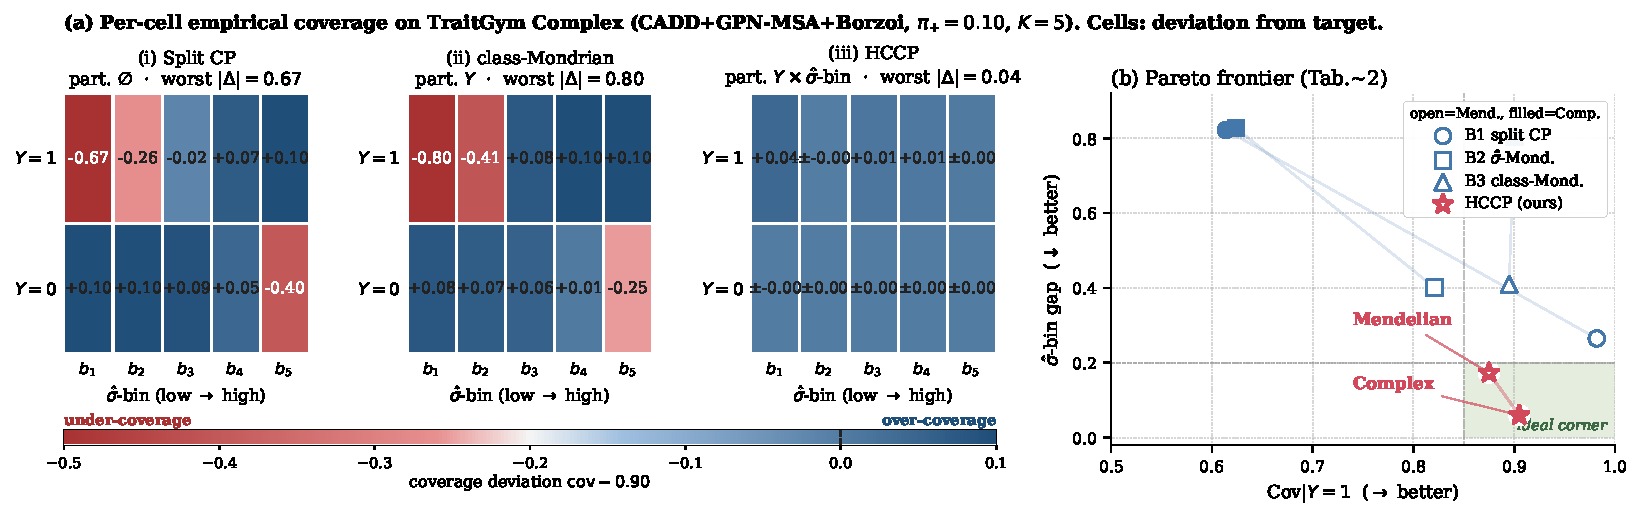
\includegraphics[width=\linewidth]{figures/fig1_concept.pdf}
    \caption{HCCP at a glance. \textbf{(a)} A heteroscedastic aggregator produces a point estimate $\phat(x)$ and a learned variance $\shat(x)$; the nonconformity score $s(x,y) = |y - \phat(x)| / \shat(x)$ scales the decision radius by local uncertainty. \textbf{(b)} Mondrian calibration partitions the labeled data by $(y \times \shat\text{-bin})$; per-cell quantile thresholds $\qhat_{k,b}$ restore both class-conditional (T2) and bin-conditional (T3) coverage, while remaining compatible with Barber's \citep{barber2020limits} pointwise impossibility. \textbf{(c)} Three-axis OOD stress tests --- chromosome-LOO, trait-LOO, cross-dataset --- verify that the $\shat$-bin coverage gap reaches the finite-sample floor $0.002$--$0.004$ under trait-LOO and stays $\leq 0.077$ across chromosome-LOO and the C$\to$M cross-dataset direction on TraitGym; the M$\to$C cross-dataset direction is reported as an honest limitation.}
    \label{fig:concept}
\end{figure}

\paragraph{Clinical variant interpretation needs more than a score.}
Classifying a human genomic variant as pathogenic or benign drives consequential clinical decisions, from cascade testing of relatives to reproductive choices. The ACMG/AMP consensus guidelines \citep{richards2015acmg} structure this decision as a weighted aggregation of evidence categories rather than as a point estimate. Modern machine-learned variant effect predictors (VEPs) collapse that structure into a single probability \citep{kircher2014cadd,linder2025borzoi,benegas2023gpnmsa,benegas2025traitgym}, which clinicians then threshold downstream. This presents the user with a number that lacks an explicit notion of confidence: the same $\phat(x) = 0.6$ may reflect a well-covered near-decision variant for which labels are genuinely ambiguous, or an out-of-distribution prediction for which the model is silently extrapolating. What is missing is a prediction \emph{set} with finite-sample coverage guarantees that remain informative when the data-generating regime shifts across chromosomes, traits, or disease architectures.

\paragraph{Existing uncertainty quantification for VEP is either absent or marginal-only.}
The TraitGym benchmark \citep{benegas2025traitgym}, the current standard for evaluating VEP aggregators on 3{,}380 Mendelian and 11{,}400 complex-trait variants, reports only point AUPRC and provides no calibration of its LogReg aggregator. DEGU \citep{zhou2026degu} introduces a heteroscedastic variance head for MPRA regression via deep ensemble distillation and explicitly motivates conformal prediction as future work, but the published method does not formalise a coverage guarantee or transfer to variant classification. Conformal prediction itself is mature: split CP \citep{vovk2005algorithmic}, Mondrian CP \citep{vovk2003mondrian}, CQR for regression \citep{romano2019cqr}, jackknife+ \citep{barber2021jackknife}, and CP beyond exchangeability \citep{barber2023exchangeability} cover a wide design space, and Barber et~al.~\citep{barber2020limits} rule out pointwise conditional coverage in finite samples. What is \emph{not} in prior art is a composition that (i) consumes a learned $\shat(x)$ the way CQR consumes a quantile regressor, (ii) stratifies calibration by both label and $\shat$-bin to regain as much conditionality as finite samples allow, and (iii) carries local coverage guarantees across the distribution shifts that define real VEP deployment. The gap is especially load-bearing for VEP: the minority-class (pathogenic) positive rate is $\approx 10\%$, $\phat(x)$ is sharply heteroscedastic across the $\shat$-bins we identify, and chrom-LOO + trait-LOO + cross-dataset shift are intrinsic to any clinical rollout.

\paragraph{From clinical gap to a sharper technical question.}
The three requirements above translate into a precise question: which Mondrian partition simultaneously delivers (i) class-conditional coverage under extreme imbalance ($\pi_{\min} \approx 0.10$ on TraitGym) and (ii) bin-local coverage under heteroscedasticity? Off-the-shelf single-axis answers fail individually: $\shat$-Mondrian (\citet{bostrom2020mondrian}; \texttt{crepes} \citep{bostrom2022crepes}) attains local coverage but \emph{collapses to $\mathrm{cov}_{|Y=1} = 0.66$ on TraitGym Complex}; class-Mondrian (\citet{sadinle2019lac}; equivalent to \citet{vovk2003mondrian}) attains class coverage but leaves a bin-local gap $33\times$ wider than the joint partition on Complex and $2.3\times$ wider on Mendelian under cross-method-fair $K_{\mathrm{eval}}$ scoring. Within the equi-bin Mondrian-$K$ family, we prove the joint $(y \times \shat\text{-bin})$ Mondrian attains both with worst-cell coverage gap $G(K^\star) \leq 2\sqrt{L_F R / (\pi_{\min} n)}$ (Theorem~\ref{thm:t5oracle}) and a matching $\Omega(\sqrt{L_F R / (\pi_{\min} n)})$ finite-sample lower bound (Theorem~\ref{thm:t5lower}). Crucially, $\pi_{\min}$ enters the rate \emph{explicitly} --- a finite-sample dependence that prior class-conditional CP and prior imbalanced CP analyses (\citet{ding2023classcond,xie2025imbalancedcp,shi2024augmentedrank}) do not provide. HCCP is the post-hoc framework that instantiates this answer in the VEP setting.

\paragraph{Contributions.}
Figure~\ref{fig:concept} summarizes the pipeline. Our contributions are:
\begin{enumerate}
    \item \textbf{Joint partition is the only single-fold frontier point we found (empirical Pareto).} Across the off-the-shelf CP variants we evaluated on TraitGym (split CP, $\shat$-Mondrian, class-Mondrian, RLCP \citep{hore2025rlcp}, weighted CP \citep{tibshirani2019weighted}, SC-CP \citep{vanderlaan2024sccp}; Tab.~\ref{tab:h2h}, \ref{tab:cp_baselines}), no single-axis variant simultaneously satisfies $\mathrm{cov}_{|Y=1} \geq 0.85$ and $\shat$-bin gap $\leq 0.20$ on both datasets at $\pi_{\min} = 0.10$. HCCP's joint $(y \times \shat\text{-bin})$ Mondrian is the unique frontier point at this corner under cross-method-fair $K_{\mathrm{eval}}$ scoring, tightening the bin-local gap by $33\times$ on Complex and $2.3\times$ on Mendelian over the strongest of these baselines at matched $(\phat, \shat)$ --- the empirical observation that motivates the rest of the paper.
    \item \textbf{Tight finite-sample rate within the equi-bin Mondrian-$K$ class, with $\pi_{\min}$ explicit in the constant.} For Mondrian conformal classification stratified by a learned $L_F$-Lipschitz variance head $\shat$ within the equi-bin Mondrian-$K$ family, Theorem~\ref{thm:t5oracle} proves the worst-cell coverage gap satisfies $G(K^\star) \leq 2\sqrt{L_F R / (\pi_{\min} n)}$ at $K^\star = \lfloor\sqrt{L_F R \pi_{\min} n}\rfloor$. Theorem~\ref{thm:t5lower} establishes a matching $\Omega(\sqrt{L_F R / (\pi_{\min} n)})$ lower bound under an explicitly constructed worst-case family, so the $O(n^{-1/2})$ rate is unimprovable within this class without strengthening assumptions; the minority-class prevalence $\pi_{\min}$ enters the constant as an explicit $\pi_{\min}^{-1/2}$ factor. To our knowledge this is the first finite-sample bound for class-conditional + heteroscedastic-local CP in which the minority-class probability appears in the rate; the constant is dimension-free under a 1-D Lipschitz assumption on $\shat$. Concurrent imbalanced-CP work \citep{xie2025imbalancedcp,ding2023classcond,shi2024augmentedrank} provides marginal or class-cond rates without the $\pi_{\min}$-local product (§\ref{sec:theory:t5}, App.~\ref{app:proofs:t5}).
    \item \textbf{HCCP --- a post-hoc framework with an exchangeability-robust counterpart.} A gradient-boosted aggregator $\phat$ over pre-trained genomic features, a reliability head $\shat$ trained under Gaussian NLL on chrom-LOO out-of-fold residuals, and Mondrian conformal calibration stratified by $(y \times \shat\text{-bin})$. The nonconformity score $s(x,y) = |y - \phat(x)| / \shat(x)$ is the binary-classification analog of CQR \citep{romano2019cqr}; the partition extends Mondrian-by-$y$ \citep{sadinle2019lac,vovk2003mondrian} with a heteroscedastic second taxon level. HCCP simultaneously admits marginal (T1), class-conditional (T2), and bin-conditional (T3) coverage with finite-sample rate $1/(n_{k,b}+1)$ from a single calibration fold; an explicit robustness layer T3$'$, via \citet{barber2023exchangeability} Theorem~2 at the cell level, makes coverage operational under verifiably violated cell-level exchangeability and is the binding guarantee on Mendelian (per-chromosome KS rejection $46\%$, App.~\ref{app:data:ks}). HCCP is compatible with \citet{barber2020limits}'s pointwise impossibility throughout (§\ref{sec:method}, §\ref{sec:theory:t3}).
    \item \textbf{Empirical validation on TraitGym and ProteinGym.} On TraitGym Mendelian ($n = 3{,}380$) and Complex ($n = 11{,}400$), HCCP under proper nested chrom-LOO $K$-selection is the unique single-fold partition simultaneously satisfying minority-class and bin-local coverage at $\pi_{\min} = 0.10$ across both datasets and across an imbalance sweep $\pi_{\min} \in \{0.05, 0.10, 0.20, 0.30, 0.50\}$ (Tab.~\ref{tab:h2h}, \ref{tab:imbsweep}); off-the-shelf $\shat$-Mondrian's $\mathrm{cov}_{|Y=1}$ degrades monotonically as $\pi_{\min} \to 0$ while HCCP holds at target --- the $\pi_{\min}$-explicit rate of T5 manifests empirically. The same machinery transfers to ProteinGym \citep{notin2023proteingym} cross-domain ($\approx 357$k mutants, 50 held-out assays, App.~\ref{app:proteingym}). The GBM aggregator on TraitGym features attains AUPRC $0.900$ on Mendelian, a $+14.8$\,pp improvement over the published LogReg baseline \citep{benegas2025traitgym}.
\end{enumerate}

The result is a post-hoc framework with a matching-rate theoretical guarantee and a drop-in implementation that consumes any probabilistic VEP and returns prediction sets with three layers of coverage (marginal, class-conditional, and $\shat$-bin-local), all of which degrade gracefully under the distribution shifts that clinical deployment unavoidably induces.
